%%%--- Template for master thesis at SfS
%%%--- Modified template with more comments and examples -- SG, 11/06/09
%%%------
\documentclass[11pt,a4paper,twoside,openright]{report}
%%not needed \usepackage{E}
\usepackage[utf8]{inputenc}
\usepackage[english]{style/ETHDAsfs}%--> ETHDASA + fancyheadings + ... "umlaute"
%  + sfs-hyper -> hyperref

\usepackage{pdfpages}%%to include the confirmation of originality (plagiarism
\usepackage{amsbsy}%% for \boldsymbol and \pmb{.}
\usepackage{amssymb}%% calls  amsfonts...
\usepackage{booktabs} % For \toprule etc. in tables
\usepackage[table]{xcolor} 
%or \usepackage{german8}%-- =  german  +  isolatin1
\usepackage{graphicx}%-- f?r PostScript-Grafiken (besser als  psfig!)
%\usepackage[draft]{graphicx} % grafics shown as boxes --> faster compilation
%
\usepackage[longnamesfirst]{natbib}%was {sfsbib}%- F?r  Literatur-Referenzen
%           ^^^^^^^^^^^^^^ 1) "Hampel, Ronchetti, ..,"  2) "Hampel et al"
% Engineers (and other funny people) want to see [1], [2]
% ---> use 'numbers' : \usepackage[longnamesfirst,number]{natbib}
%
%
\usepackage{style/texab}%- 'tex Abk?rzungen' /u/sfs/tex/tex/latex/texab.sty
        %%- z.B.  \R, \Z, \Q, \Nat f?r reelle, ganze, rationale, nat?rl. Zahlen;
        %%-       \N   (Normalvert.)  \W == Wahrscheinlichkeit .....
        %%-  \med, \var, \Cov, \....
        %%-  \abs{x} == |x|   und   \norm{y} ==  || y ||   (aber anst?ndig)
%% NOTE: texab contains many useful definitions and "shortcuts". It is
%% worth to open the file and have a look at them. HOWEVER, some
%% definitions can lead to conflicts with other packages. You
%% might for example want to comment out the line defininf \IF as an
%% operator when working with the algorithmic package, or to comment out
%% the line defining a command \Cite with working with the Biblatex package
\usepackage{amsmath}
%\usepackage{mathrsfs}% Raph Smith's Formal Script font --> provides \mathscr
\usepackage{enumerate}% Fuer selbstdefinierte Nummerierungen
\usepackage{longtable}
%--------
\usepackage{relsize}%-> \smaller (etc) used here
\usepackage{color} %% to allow cloring in code listings
\usepackage{listings}% Fuer R-code, C-code, ....  and settings for these:
\definecolor{Mygrey}{gray}{0.75}% for linenumbers only!
\definecolor{Cgrey}{gray}{0.4}% for comments
\lstloadlanguages{R}
\lstset{ %% Hilfe unter z.B. http://en.wikibooks.org/wiki/LaTeX/Packages/Listings
language=R,
basicstyle=\ttfamily\scriptsize,%%- \small > \footnotesize > \scriptsize > \tiny
%commentstyle=\ttfamily\color{Cgrey},
commentstyle=\itshape\color{Cgrey},
numbers=left,
numberstyle=\ttfamily\color{Mygrey}\tiny,
stepnumber=1,
numbersep=5pt,
backgroundcolor=\color{white},
showspaces=false,
showstringspaces=false,
showtabs=false,
frame=single,
tabsize=2,
captionpos=b,
breaklines=true,
%breakatwhitespace=false,
keywordstyle={},
morekeywords={},
xleftmargin=4ex,
literate={<-}{{$\leftarrow$}}1 {~}{{$\sim$}}1}
\lstset{escapeinside={(*}{*)}} % for (*\ref{ }*) inside lstlistings (Scode)
%%----------------------------------------------------------------------------

%%------- Theoreme ---
\newtheorem{definition}{Definition}[subsection]
\newtheorem{lemma}[definition]{Lemma}
\newtheorem{theorem}[definition]{Theorem}
\newtheorem{Coro}[definition]{Corollary}
\theoremstyle{definition}
\newtheorem{example}[definition]{Example}
\newtheorem*{note}{Note}
\newtheorem*{remark}{Remark}

\DeclareMathOperator*{\plim}{plim}
% \def\MR#1{\href{http://www.ams.org/mathscinet-getitem?mr=#1}{MR#1}}

% \newcommand{\Lecture}[3]{\marginpar{#3.#2.#1}}
% \newcommand{\Fu}{\mathcal{F}}
\newcommand{\aatop}[2]{\genfrac{}{}{0pt}{}{#1}{#2}}

%\renewcommand{\theequation}{\arabic{equation}}
\numberwithin{equation}{subsection}

%%%%%%%%%%%%%%%%%%%%%%%%%%%%%%%%%%%%%%%%%%%%%%%%%
%%% Path for your figures                      %%%
%%%%%%%%%%%%%%%%%%%%%%%%%%%%%%%%%%%%%%%%%%%%%%%%%
% Set the paths where all figures are taken from:
\graphicspath{{images/}}

%%%%%%%%%%%%%%%%%%%%%%%%%%%%%%%%%%%%%%%%%%%%%%%%%
%%% Define your own commands here             %%%
%%%%%%%%%%%%%%%%%%%%%%%%%%%%%%%%%%%%%%%%%%%%%%%%%
\newcommand{\Bruch}[2]{{}^{#1}\!\!/\!_{#2}}
\renewcommand{\labelenumi}{\roman{enumi}.)}
\providecommand{\tightlist}{%
  \setlength{\itemsep}{0pt}\setlength{\parskip}{0pt}}

\makeatletter
\@ifundefined{Shaded}{
}{\renewenvironment{Shaded}{\begin{kframe}}{\end{kframe}}}
\makeatother
\usepackage{color}
\usepackage{fancyvrb}
\newcommand{\VerbBar}{|}
\newcommand{\VERB}{\Verb[commandchars=\\\{\}]}
\DefineVerbatimEnvironment{Highlighting}{Verbatim}{commandchars=\\\{\}}
% Add ',fontsize=\small' for more characters per line
\usepackage{framed}
\definecolor{shadecolor}{RGB}{248,248,248}
\newenvironment{Shaded}{\begin{snugshade}}{\end{snugshade}}
\newcommand{\AlertTok}[1]{\textcolor[rgb]{0.94,0.16,0.16}{#1}}
\newcommand{\AnnotationTok}[1]{\textcolor[rgb]{0.56,0.35,0.01}{\textbf{\textit{#1}}}}
\newcommand{\AttributeTok}[1]{\textcolor[rgb]{0.13,0.29,0.53}{#1}}
\newcommand{\BaseNTok}[1]{\textcolor[rgb]{0.00,0.00,0.81}{#1}}
\newcommand{\BuiltInTok}[1]{#1}
\newcommand{\CharTok}[1]{\textcolor[rgb]{0.31,0.60,0.02}{#1}}
\newcommand{\CommentTok}[1]{\textcolor[rgb]{0.56,0.35,0.01}{\textit{#1}}}
\newcommand{\CommentVarTok}[1]{\textcolor[rgb]{0.56,0.35,0.01}{\textbf{\textit{#1}}}}
\newcommand{\ConstantTok}[1]{\textcolor[rgb]{0.56,0.35,0.01}{#1}}
\newcommand{\ControlFlowTok}[1]{\textcolor[rgb]{0.13,0.29,0.53}{\textbf{#1}}}
\newcommand{\DataTypeTok}[1]{\textcolor[rgb]{0.13,0.29,0.53}{#1}}
\newcommand{\DecValTok}[1]{\textcolor[rgb]{0.00,0.00,0.81}{#1}}
\newcommand{\DocumentationTok}[1]{\textcolor[rgb]{0.56,0.35,0.01}{\textbf{\textit{#1}}}}
\newcommand{\ErrorTok}[1]{\textcolor[rgb]{0.64,0.00,0.00}{\textbf{#1}}}
\newcommand{\ExtensionTok}[1]{#1}
\newcommand{\FloatTok}[1]{\textcolor[rgb]{0.00,0.00,0.81}{#1}}
\newcommand{\FunctionTok}[1]{\textcolor[rgb]{0.13,0.29,0.53}{\textbf{#1}}}
\newcommand{\ImportTok}[1]{#1}
\newcommand{\InformationTok}[1]{\textcolor[rgb]{0.56,0.35,0.01}{\textbf{\textit{#1}}}}
\newcommand{\KeywordTok}[1]{\textcolor[rgb]{0.13,0.29,0.53}{\textbf{#1}}}
\newcommand{\NormalTok}[1]{#1}
\newcommand{\OperatorTok}[1]{\textcolor[rgb]{0.81,0.36,0.00}{\textbf{#1}}}
\newcommand{\OtherTok}[1]{\textcolor[rgb]{0.56,0.35,0.01}{#1}}
\newcommand{\PreprocessorTok}[1]{\textcolor[rgb]{0.56,0.35,0.01}{\textit{#1}}}
\newcommand{\RegionMarkerTok}[1]{#1}
\newcommand{\SpecialCharTok}[1]{\textcolor[rgb]{0.81,0.36,0.00}{\textbf{#1}}}
\newcommand{\SpecialStringTok}[1]{\textcolor[rgb]{0.31,0.60,0.02}{#1}}
\newcommand{\StringTok}[1]{\textcolor[rgb]{0.31,0.60,0.02}{#1}}
\newcommand{\VariableTok}[1]{\textcolor[rgb]{0.00,0.00,0.00}{#1}}
\newcommand{\VerbatimStringTok}[1]{\textcolor[rgb]{0.31,0.60,0.02}{#1}}
\newcommand{\WarningTok}[1]{\textcolor[rgb]{0.56,0.35,0.01}{\textbf{\textit{#1}}}}

\begin{document}
\bibliographystyle{style/chicago}% ---> Hampel,F., E.Ronchetti,... W.Stahel(1986) ...
 %was \bibliographystyle{sfsbib}\citationstyle{dcu} %OR DEFAULT : \citationstyle{agsm}

\pagenumbering{roman}%- roman numbering for first few pages

%%%%%%%%%%%%%%%%%%%%%%%%%%%%%%%%%%%%%%%%%%%%%%%%%
%%% Title page                                %%%
%%%%%%%%%%%%%%%%%%%%%%%%%%%%%%%%%%%%%%%%%%%%%%%%%
\period{April 2018}
\dasatype{Master Thesis}
\students{Nicola Gnecco and Lorenz Walthert}
\alternatereaderprefix{Adviser:}
\alternatereader{Prof.~Dr.~Nicolai Meinshausen}
\mainreaderprefix{}
\mainreader{}


\submissiondate{August 1th 2018}
\title{A bookdown template for sfs}

\maketitle%- Titelseite wird abgeschlossen
\cleardoublepage
 %%~~~~~~~~~~~~~~~~~~~~~~~~~~~~~~~~~~~~~~~~

%%%%%%%%%%%%%%%%%%%%%%%%%%%%%%%%%%%%%%%%%%%%%%%%%
%%% Insert here acknowledgements and abstract %%%
%%%%%%%%%%%%%%%%%%%%%%%%%%%%%%%%%%%%%%%%%%%%%%%%%
%% Dedication (optional)
\markright{}
\vspace*{\stretch{1}}
\begin{center}
    To some special person
\end{center}
\vspace*{\stretch{2}}

% Preface (optional)
\newpage
\markboth{Preface}{Preface}
\chapter*{Preface}

I would like to extend my gratitude to all the people that supported me throughout the this project. To Matthias, that from the start of my interest in this field, inspired and challenged me to create something new. You taught me many lessons that will stay with me and I value enormously the interesting conversations that stimulated a lot of excitment and creativity. To Maybritt, thank you for your support, insights, supervision and the many conversations that inspired solutions. Your encouragements from the start to the end were incredibily valuable. To Belinda, your help was essential in fortifying my physics competences and I appreciated the time you spend supporting my work. To Heini, thank you for the supervision and feedback that was instrumental in shaping a meaningul and impactful project. You all showed interest in my work and I am very grateful to have had such a competent, enthusiastic and friendly team.

This thesis has been a unique opportunity to place myself at the head of a scientific project, and it was foremost a humbling experience, as the challenges of interdisplinary research have taught me. Throughout all the ups and down, I would like to thank my friends for the moments of laughter, for being great rubber ducks, and for all the good times. I will miss you all a lot and am eager to follow all your future adventures. Grazie mamma per essere stata sempre raggiungibile, per le poesie ispirante e le foto del grigio che mi fanno sorridere molto. Merci papa pour ces parties de ping-pong qui me sont si importantes et les bons verres de vins. To Matt and Luca, always wonderful to have you around: I cherish all the moments we have together. To my Manu, thank you for everything. Your calls and visits brought me joy and comfort, our time together is so dear to me and you are always an inspiration. I am so glad to have you by my side. 


%%% Local Variables: 
%%% mode: latex
%%% TeX-master: "MasterThesisSfS"
%%% End: 


% Abstract should not be longer than one page.
\newpage
\markboth{Abstract}{Abstract}
\chapter*{Abstract}

Heat-related extremes are important meteorological phenomena that can have strong consequences on human health and the environment. Climate change is expected to exacerbate these impacts through an increase in the frequency of hot extreme occurrence and intensity. Although there exists abundant literature on the typical physical functioning of these events and their association to the variability of the climate system on different temporal scales, there lacks a global assessment of the influence of major physical processes - heat advection, adiabatic compression and diabatic heating - on the yearly variation of hot extreme magnitudes. To remediate this knowledge gap, we first propose a data-driven, systematic analysis of second-moment characteristics of yearly maxima near-surface hot extreme events and contributing heat-generating processes. Second, we apply deep-learning methods to model hot extreme Lagrangian trajectories to gain insights into important dynamical features. No physical process is globally found to dominate variability in these events and significant variance contributions exist from at least two processes, suggesting that mean-state understanding of hot extreme development may not not be sufficient to explain large year-to-year differences in their magnitudes. Furthermore, this analysis reaffirms the presence of strong dependencies between the three physical mechanisms leading to a characterization of their variability by only one or two degrees of freedom in most of the world. Finally, the approach for the analysis of parcel trajectories was limited due to generally poor predictive performance, but showed that the patterns in advective, adiabatic and diabatic temperature anomaly generation follow patterns that may be predicted from their history, encouraging for future work. In addition, over oceans and many land regions we observe that adiabatic heating is minimal during the final 24h, suggesting that hot extreme primarily descend to the surface earlier than a day before, thus leading to contributions from advective and diabatic processes more likely.

%%% Local Variables: 
%%% mode: latex
%%% TeX-master: "MasterThesisSfS"
%%% End: 



%%%%%%%%%%%%%%%%%%%%%%%%%%%%%%%%%%%%%%%%%%%%%%%%%
%%% Table of contents and list of figures and %%%
%%% tables (no need to change this usually)   %%%
%%%%%%%%%%%%%%%%%%%%%%%%%%%%%%%%%%%%%%%%%%%%%%%%%
\newpage
\tableofcontents
\newpage
\listoffigures
\newpage
\listoftables

%% Notations and glossary (optional)
\cleardoublepage
\phantomsection

\markboth{Notation}{Notation}
\chapter*{Notation}
\label{c:Notation}

Explain your symbols and abbreviations.

%%% Local Variables: 
%%% mode: latex
%%% TeX-master: "MasterThesisSfS"
%%% End: 


\cleardoublepage
\pagenumbering{arabic}%--- switch back to standard numbering


%%%%%%%%%%%%%%%%%%%%%%%%%%%%%%%%%%%%%%%%%%%%%%%%%
%%% Your text... Either write here directly,  %%%
%%% or even better: write in separate files   %%%
%%% that you just have to include here.       %%%
%%%%%%%%%%%%%%%%%%%%%%%%%%%%%%%%%%%%%%%%%%%%%%%%%
\hypertarget{a-few-words-from-the-authors}{%
\chapter*{A few words from the authors}\label{a-few-words-from-the-authors}}


This repository is a \href{https://github.com/rstudio/bookdown}{bookdown} template,
derived from the LaTeX template from the seminar for statistics, ETH Zurich.

\textbf{How bookdown works}

In a nutshell, bookdown works as follows:

\begin{itemize}
\tightlist
\item
  use knitr to convert Rmd to markdown.
\item
  use pandoc to convert markdown to latex, pdf, word, html books (with features
  like font size, background selection, full text search etc), epub.
\end{itemize}

The basic workflow in RStudio is as follows:

\begin{itemize}
\tightlist
\item
  Open the RStudio project.
\item
  Change a source file: In our template, the source of the body of the thesis
  is under \texttt{./rmd/}. For example, change \texttt{02-features.Rmd}. To make sure only
  files from this directory are used, we set the option \texttt{rmd\_subdir:\ {[}"rmd/"{]}}
  in \texttt{bookdown.yml}. For this to work you need bookdown version 0.9 or greater.
\item
  Re-compile the book using Cmd + Shift + B (for build) on a Mac and Ctrl +
  Shift + B on Windows / Linux.
\item
  You can customize the build in the RStudio Build Tab, where you can specify
  which output (html, pdf, etc.) you want to generate. This is remembered for the
  next build you are doing.
\end{itemize}

\textbf{Getting started}

For the git cracks: Fork the upstream repository and clone the fork.Then, you will have one remote
repository: origin, which refers to the fork. Add the upstream repo as an
upstream remote so you can later rebase on it in case you need. We recommend
using ssh over https, but if that's too complicated with the RSA key, just
use https, it will do the job.

For everyone else: You can also simply download the repo.
However, we strongly recommend using version control for your thesis.

Make sure to \href{https://help.github.com/en/articles/watching-and-unwatching-repositories}{watch}
this GitHub repo for issues that might affect you.

\textbf{Why using bookdown}

The advantages of using bookdown instead of plain LaTeX are, in the eyes of the
creator of this template:

\begin{itemize}
\tightlist
\item
  Generalization. Not just latex or PDF output, but any output supported by
  Pandoc, e.g.~Word and html, epub. If you at some point decide to work with
  LaTeX only, just render to LaTeX and continue. You don't loose anything
  compared to status quo. When you host your source code on GitHub, you can
  easily publish a html book that is updated with every push. How? Checkout
  \url{https://github.com/ropenscilabs/tic.bookdown}.
\item
  The best of two worlds. Use intuitive markdown syntax where possible, use the
  full power of LaTeX syntax where needed. This includes bibtex reference, LaTeX
  cross-, text- and figure reference.
\item
  It's native R. Integrate R code and R output such as plots, tables, figures
  directly in your writing has never been easier than with bookdown. You can turn
  a data frame into a latex table using the power of R packages such as
  \texttt{kableExtra}. You can change the data subset, re-compile the whole book and
  all figures, tables and other data dependent elements will be updated.
\item
  The power of RStudio. Use the same IDE for programming and writing. Leverage
  the advantages of a real-time latex equation previewer right in your R
  Markdown, a git GUI, spell checking, file browser and more.
\item
  You can also use other languages supported by knitr such as
  python, stan etc. You can even use R code to control the behavior of chunk
  evaluation. Below, we even used the bash command \texttt{tree} to show the
  directory structure of this repo. Since unicode is not supported with pdflatex,
  we used R code to tell knitr to use the tree command with the option \texttt{charset\ \ \ unicode} for pdf output and without it for html output. Check the Rmd source
  of the README to learn more.
\item
  Because it's native R, you can place R variables in the floating text. Check
  out the Rmd source of this document to see that we used R to compute the square
  root of three (1.7320508), print today's date with \texttt{Sys.Date()} right into the
  text: 2024-07-31
\end{itemize}

\textbf{How this template works}

There are different directories in this template:

\begin{Shaded}
\begin{Highlighting}[]
\ExtensionTok{tree} \AttributeTok{{-}d} \AttributeTok{{-}L}\NormalTok{ 2 }\AttributeTok{{-}{-}charset}\NormalTok{ unicode}
\end{Highlighting}
\end{Shaded}

\begin{itemize}
\tightlist
\item
  \_book: Contains the compiled book, e.g.~a PDF or html version.
\item
  \_bib: Contains BibTeX reference data bases.
\item
  figure: Contains figures you created from your (R) code in the rmd source.
\item
  images: Put images you want to include in your thesis in this folder.
\item
  pdf: Put PDFs you want to include in your thesis in this folder.
\item
  rmd: The source folder of thesis. When you build a book, the following
  happens: By default, all rmd files in this folder get merged into one big rmd
  file, according to their name. We suggest to use one file per chapter. Then, the
  file containing all the rmd sources will get processed by knitr and later by
  Pandoc.
\item
  scratch: A random directory which is not tracked by git by default. The idea
  is that you can put things that are not ready to commit or that have a temporary
  character here.
\item
  style: Latex .sty files. Taken from the sfs LaTeX template.
\item
  tex: All tex data, most importantly, the sfs LaTeX template itself. Note that
  the abstract, preface, epilogue, summary, notation are still in tex, i.e.~you
  need to change these files if you want the PDF output to change. This will
  \textbf{not} affect the html output. You can create chapters that show up in a
  particular output and not in the other forms as shown in
  \texttt{rmd/99-references.Rmd}.
\end{itemize}

Furthermore, we want to highlight a few files in the root directory of the
project:

\begin{itemize}
\tightlist
\item
  \texttt{DESCRIPTION}: You can use it to declare dependent packages of your thesis in
  the \texttt{Imports:} field. If someone want's to rebuild you thesis from scratch, the
  can use \texttt{remotes::install\_deps()} to satisfy all R package dependencies.
\item
  \texttt{index.Rmd}: Contains a YAML header where a few important variables are
  defined. You can also put markdown below the header.
\item
  \texttt{README.(R)md}: This document.
\item
  \texttt{thesis-template-bookdown.Rproj}: An RStudio project. We recommend using
  RStudio for authoring your master thesis with bookdown.
\end{itemize}

\textbf{A few recommendations}

\begin{itemize}
\tightlist
\item
  We strongly suggest to use a different folder for the data / code of your
  thesis and reserve this directory for the thesis document only. You can rename
  this directory \texttt{analysis-communication} (since this will be the means used for
  communicating the results and process of your thesis) and use \texttt{analysis-raw} for
  the code and \texttt{data} for all data. Ideally, you place them in the same directory
  so you can still work with relative paths, e.g.~\texttt{../data}.
\item
  We suggest to use the package manager \href{https://rstudio.github.io/renv/}{\{renv\}}
  for better reproducibility and isolation for the packages in this project from
  the global library. It's already initialised with this template. All packages
  you install and update are contained in a separate library.
\item
  We suggest to use git version control for the thesis and the raw analysis.
\item
  If your thesis is open source, you can use netlify.com to deploy it, i.e.~for
  every commit you push to a remote repo like GitHub, you can use netlify's CLI to
  build your book on a CI machine like travis. See file \texttt{travis.yml} for the
  bookdown book \href{https://github.com/hadley/adv-r/tree/88dcb07e2b2ae634af6cdeafff2f3ea976077064}{Advanced
  R}
  for an example. That makes tracking the \texttt{\_book} folder in git redundant.
\item
  To keep lines 80 characters long, you can use the stylermd Rstudio Addin.
  Assign a keyboard shortcut to it and it will format your text nicely.
  See \url{https://github.com/lorenzwalthert/stylermd} for details.
\item
  You might want to use \href{https://docs.ropensci.org/targets/}{\{targets\}}, a MAKE
  like pipelining tool to keep your analysis reproducible and only re-execute
  the outdated parts.
\end{itemize}

\textbf{Further material}

This is obviously a very short introduction to the template and it is in no way
comprehensive. To learn more about bookdown, we encourage the reader to have a
look at the \href{https://bookdown.org/yihui/bookdown/}{bookdown guide} as well as
searching through stack overflow / Google for particular questions. In addition,
inspect the different files in this repo, in particular the ones in the rmd
directory to develop a deeper understanding of the template.

As of early 2018, this template is still in alpha testing phase, so you may
experience unexpected behavior. If you experience problems
\emph{after} you searched on Google and other platforms for a solution, feel free to
open an issue in this repo.

Best,

Nicola Gnecco and Lorenz Walthert

\hypertarget{introduction}{%
\chapter{Introduction}\label{introduction}}

\hypertarget{motivation}{%
\section{Motivation}\label{motivation}}

In recent years, near-surface hot extremes have globally become increasingly more important. They impact human health with often high mortality rates in certain demographics (REF, REF, REF); can be damaging to agricultural and ecological systems through productivity decreases and heat stress (Teixeira, REF, REF); and may pressure national economies by increasing energy demands (Perera) compounded with power infrastructure damage (Entricken), as well as lowering labour productivity (Garcia-Leon). Furthermore, climate change is expected to exacerbate hot extreme impacts through an increase in the frequency of hot extremes as well as their intensity (R. Slater et al., 2021; E. Fischer et al.~2021; V. Thompson et al., 2022). There is thus a need for robust process understanding of the drivers of hot extremes to guide emergency planning and mitigation strategies.

Globally, heat-waves and hot extreme events contribute the largest risks to human societies (maybe too strong, but can find a good source).

Coupled with increasing mean global temperatures, recent record-shattering events highlight the importance in understanding not only the evolution and drivers of typical hot extremes, but also their variability. The Pacific North-West 2021 event is particularly illustrative: it was hard to predict with no ensemble member resolving such intense temperature 10 days before (Hai Lin et al., 2022);

with models / forecasters not expecting temperatures that went above return period estimations (REF). Uncovering the differences that separate such events from lower-intensity hot extremes is helpful to understand how they may change under climate change.

\hypertarget{related-work}{%
\section{Related work}\label{related-work}}

In order to present a holistic review of existing literature on hot extremes, their development is examined with three heat-generating mechanisms: advection involves the horizontal transport of warmer air into a cooler air mass; adiabatic heating arises from descending air that compresses and thus heats; diabatic heating involves radiative effects and sensible heat fluxes from the Earth's surface. The absence of the reverse mechanisms (cold air advection, ascending air and diabatic cooling) may also contribute to the formation of hot extremes. This characterisation providing a uniform basis to discuss atmospheric phenomena linked to hot extreme evolution and suggests a methodology, discussed in Methods, to quantify the contribution of these physical processes to specific events.

In the mid-latitudes, the major weather regime influencing hot extremes is atmospheric blocking, a pattern characterized by persistent anticyclonic activity that prevents the influence of the prevailing flows (A. Lupo, 2020). Over Central and Western Europe, atmospheric blocking leads to regions of large subsidence and fair weather, further promoting strong radiative heating (L. Kautz, et al, 2022). Quantifying the co-location of atmospheric blocking and hot extremes has however shown large spatial variability both in the Northern (S. Pfahl and H. Wernli, 2012; L. Brunner et al., 2018) and Southern Hemisphere mid-latitudes (A. Pezza et al., 2011). WHAT ABOUT THE TROPICS. For polar latitudes, a case-study on the March 2022 East Antarctica heat extreme shows that intense atmospheric blocking led the weakening of the ice-sheet temperature inversion, intensifying adiabatic heating from subsiding air.

Soil-dryness has been shown to be both a major driver of hot extreme events as well as exacerbate atmospheric blocking condition. Soil moisture deficit is understood to increase surface sensible heat fluxes, in turn ``leading to diurnal convection favouring the entrainment of warm air, and the formation of deep and warm nocturnal residual layers allowed the heat to re-enter the mixed layer in the following days'' (D. Miralles et al., 2014). M. Vogel et al.~(2017) quantified these effects, finding that more than 70\% of increase in TX1day magnitude in Central Europe and Central North America, and around 50\% in Amazonia, Northern Australia and Southern Africa.

Marine heatwaves and TX1day events are understood to evolve \ldots{} E. Oliver et al., 2020

In addition to understanding the development of hot extremes, many studies have focused on the influence of multi- and inter-decadal variability. TO DO

Beyond understanding the mean behaviour of hot extremes, a limited number of studies have investigated the variability of hot extremes at local to regional spatial scales. Over Europe, E. Fischer and C. Schar (2008) quantified the changes in hot extreme variability with respect the processes associated with inter-annual variability, intra-seasonal variability and the seasonal variability of summer months. L. Suarez-Gutierrez et al.~(2020) instead suggests attributing variability changes to dynamical and thermodynamical sources, concluding that dynamical mechanisms, encompassing effects of atmospheric blocking, are the main drivers of hot extreme variability.

TALK ABOUT THE METHODOLOGIES USED IN OTHER EXTREME RESEARCH:
A. Casanueva et al.~(2014) propose investigating the variability of extreme precipitation events through large-scale teleconnection patterns, such as the Southern Oscillation and the North Atlantic Oscillation, by trend analysis and correlation analysis.

The weather extremes literature has used two main methodologies: trajectory analysis such as Lagrangian tools (\ldots, \ldots, \ldots) and sensitivity analysis. Trajectory analysis have been limited to `manual' stuff (no ML)

Although a good general understanding of hot extreme evolution exists and more detailed assessments have been made regionally and for specific high-impact events, there then exists a knowledge-gap in quantifying the contribution of known physical processes to hot extreme magnitude variability globally. This manuscripts attempts to close this gap by first proposing a systematic analysis of second-moment characteristics of hot extreme events and second applying state-of-the-art deep-learning methods to uncover evolutionary features influencing their magnitudes.

\hypertarget{features}{%
\chapter{Features}\label{features}}

\texttt{bookdownplus} extends the features of \texttt{bookdown}, and simplifies the
procedure. Users only have to choose a template, clarify the book title and
author name, and then focus on writing the text. No need to struggle in YAML
and LaTeX.
With \texttt{bookdownplus} users can

\begin{itemize}
\item
  record guitar chords,
\item
  write a mail in an elegant layout,
\item
  write a laboratory journal, or a personal diary,
\item
  draw a monthly or weekly or conference calendar,
\item
  and, of course, write academic articles in your favourite way,
\item
  with chemical molecular formulae and equations,
\item
  even in Chinese,
\item
  and more wonders will come soon.
\end{itemize}

Full documentation can be found in the book
\href{https://bookdown.org/baydap/bookdownplus}{R bookdownplus Textbook}. The webpage
looks so-so, while the
\href{https://bookdown.org/baydap/bookdownplus/bookdownplus.pdf}{pdf file} might give
you a little surprise.

\hypertarget{methods}{%
\chapter{Methods}\label{methods}}

\hypertarget{decomposition-of-tx1day-anomalies-and-their-yearly-variance}{%
\section{Decomposition of TX1day anomalies and their yearly variance}\label{decomposition-of-tx1day-anomalies-and-their-yearly-variance}}

To this end, we focus on investigating yearly maxima of 1-day temperature anomaly averages, denoted TX1day. Using anomalies, rather than magnitudes, leads to a more natural interpretation of the components' contribution to extreme warming, since some processes of interest, such as warming from horizontal advection, arise due to climatological differences *** (explain better). The variation in TX1day and its relation to underlying physical processes is captured by using the decomposition of TX1day anomalies into contributions from horizontal advection, adiabatic warming and diabatic warming (1), according to M. Rothlisberger and L. Papritz (2023). These quantities are now referred to as the advective (adv), adiabatic (adiab) and diabatic (diab) temperature anomalies. The decomposition is derived with a Lagrangian perspective, meaning that it diagnostically evaluates the evolution of a parcel of air along its trajectory in 3D space and time.

At location \(\mathbf{x}\) and some time \(t_X\), the temperature anomaly \(T'\) may be decomposed as follows:

\begin{equation}
\label{eq:1}
 \begin{split}
   T'(\mathbf{x},t_X)  & = - \int_{t_g}^{t_X} \frac{\partial \bar{T}}{\partial t} \, \text{d}\tau - \int_{t_g}^{t_X} \mathbf{\nu} \mathbf{\nabla}_h \bar{T} \, \text{d}\tau + \int_{t_g}^{t_X} \left[ \frac{\kappa T}{p} - \frac{\partial \bar{T}}{\partial p}\right] \omega \, \text{d}\tau + \int_{t_g}^{t_X} \left( \frac{p}{p_0} \right)^\kappa \frac{\text{D}\theta}{\text{D}t} \, \text{d}\tau   \\
   & = \qquad \text{seas} \qquad \, + \, \quad \quad \text{adv} \qquad \, \, + \qquad \qquad \text{adiab} \qquad \quad \,  + \qquad \quad \text{diab} 
\end{split}
\end{equation}

where \(\bar{T}\) the temperature climatology; \(t_g < t_X\) genesis time, the time at which \(T'\) was last zero; \(\mathbf{\nu}\) the horizontal wind velocity; \(\mathbf{\nabla}_h\) the horizontal temperature gradient; \(p\) pressure; \(\omega\) vertical velocity; \(\theta\) potential temperature.

To apply this decomposition for the study of hot extremes, LAGRANTO is employed to compute back-trajectories of air parcels found near the surface of a location of a hot extreme event. Given data described section 3, for each year at each location, a total of 24 back-trajectories are obtained corresponding to the 3 lower model-levels for 8 timesteps with 3 hour intervals. Each trajectory is computed until genesis \(t=t_g\) of the temperature anomaly of the parcel, up to a maximum of 120 time-steps. The final dataset is created by evaluating the integrals for each of the 24 trajectories and taking an average of the final decomposed temperature anomaly.

Evaluating the integrals involves two errors arising from discrete approximations of the continuous time domain: error 1 denotes the deviation from zero of \(T'(\cdot ,t_g)\); error 2 denotes the remainder of the components, seasonality and error 1 subtracted from \(T'\). These errors are usually small relative to hot extreme \(T'\) magnitudes and are thus dropped from further analysis. In addition, since TX1day events evolve on sub-seasonal timescales, the seasonality term (seas) is small and is also dropped. These decisions are supported by Appendix A.

To extend the study of mean-behaviour of TX1day events by M. Rothlisberger and L. Papritz (2023), we propose a variance decomposition of temperature anomaly that quantifies the contributions of physical processes on variability. For \(n\) temperature anomaly samples \(\{ T' \}_{1:n}\) assuming that \$T'\_i = \$ adv\(_i +\) adiab\$\_i + \$ diab\(_i\), we have that:

\begin{equation}
\label{eq:2}
 \begin{split}
   V(\{ T' \}_{1:n})  & = V(\{ \text{adv} \}_{1:n} ) + V(\{ \text{adiab} \}_{1:n} ) + V(\{ \text{diab} \}_{1:n} ) + \\
   & \qquad Cov(\{ \text{adv} \}_{1:n} ,\{ \text{adiab} \}_{1:n}) + Cov(\{ \text{adv} \}_{1:n},\{ \text{diab} \}_{1:n}) + Cov(\{ \text{adiab} \}_{1:n},\{ \text{diab} \}_{1:n})
\end{split}
\end{equation}

Applying \ref{eq:2} to every location on Earth yields a direct and systematic approach to the analysis of global patterns of hot extreme variability in the presence of complex dependencies between physical processes. The linearity of the covariance operator and the fact that it is un-normalized, in comparison to correlation for instance, allows for a more intuitive comparison of second-moment contributions.

\hypertarget{principle-component-analysis}{%
\section{Principle Component Analysis}\label{principle-component-analysis}}

Principle Component Analysis (PCA), known as Empirical Orthogonal Functions in climate sciences, is a linear transformation introduced by K. Pearson (1901) and first applied in climate sciences for weather prediction by E. Lorenz (1956). Given multivariate samples of dimension \(p\), it expresses data into \(p\) orthogonal linear combinations of the original coordinates, determined iteratively to maximize explained variance. It is commonly used as a dimension reduction method by truncating to coordinates with high explained variance and in machine learning to yield data with uncorrelated features.

We employ PCA to investigate the dependence structure of the temperature anomaly decomposition. Similar to the variance decomposition, the transform is applied independently to series of yearly maxima TX1day events at every location on Earth with the aim of providing insights in spatial variability.

\hypertarget{baselines-for-trajectory-data}{%
\section{Baselines for trajectory data}\label{baselines-for-trajectory-data}}

As was earlier discussed, trajectory-based analyses are often carried out case-by-case and thus difficult to systematically apply for a global study. We propose leveraging the flexibility of machine learning models to investigate trajectories of yearly maxima TX1day decompositions. To compare the predictive performance of the state-of-the-art model introduced in the next section, X standard baseline models are employed: constant final-value, a Long Short-Term Memory (LSTM) network and a Gated Recurrent Unit (GRU) network.

LSTMs and GRUs are types of Recurrent Neural Networks (RNN) using feedback loops to allow outputs of one cell to be the inputs of a subsequent cell. LSTMs were introduced by Hochreiter and Schmidhuber (1997) to solve vanishing gradients in applications with long-term dependencies. Each LSTM layer is composed of three gates - the input, forget and output gates - that are recurrently computed one timestep at a time to update temporal relationships, expressed in current and hidden states. This complex structure implies considerable model flexibility, but is prone to over-fitting. GRUs are introduced by \ldots{} to reduce the number of model parameters by utilizing only two gates per recurrence. Figure X illustrates the architecture and the relevant equations.

These models are applied to timeseries obtained by averaging back-trajectories integrated from genesis \(t_g\) to times \(t_{g+1}\), \(t_{g+2}\), \ldots, \(t_{0}\), where the final time is the last timestep before the day of the hot extreme. RNN architectures learn temporal patterns by \ldots{} and we therefore augment the data by applying a sliding window to each timeseries.

Talk about cross-validation technique or parameter selection.

Talk about used loss function

Talk about validation: we want it to be good at predicting 4 steps forward, but especially the final timesteps. Maybe a weighted loss? Could use this:
\url{https://www.ncbi.nlm.nih.gov/pmc/articles/PMC7038523/}

\hypertarget{shapelet-based-neural-networks}{%
\section{Shapelet-based neural networks}\label{shapelet-based-neural-networks}}

\hypertarget{data}{%
\chapter{Data}\label{data}}

We apply the aforementioned methodologies to ERA5 data with \(0.5^{\circ} \times 0.5^{\circ}\) horizontal resolution, 137 vertical coordinates expressed as model-levels and 3-hour temporal resolution from 1980 to 2020. The coarser resolution from the full ERA5 product is required as variables such as \ldots{} are reported only in the chosen resolution. In addition, the computational costs of running multiple LAGRANTO back-trajectories per grid cell per year are limiting.

\hypertarget{quick-start}{%
\chapter{Quick start}\label{quick-start}}

Although this section might not be the latest version, the general idea won't
change. Please see
\href{https://bookdown.org/baydap/bookdownplus}{R bookdownplus Textbook} to keep up
with the update.

\hypertarget{preparation}{%
\section{Preparation}\label{preparation}}

Before starting, you have to install R, RStudio, bookdown package, and
other software and packages (i.e.~Pandoc, LaTeX, rmarkdown, rticle,
knitr, etc.) which bookdown depends on. See the official
\href{https://bookdown.org/yihui/bookdown/}{manual} of bookdown for details.
Additionally, if you want to produce a poster, phython must be installed before
using, and the path of phython might have to be added to the environmental
variables for Windows users.

\hypertarget{installation}{%
\section{Installation}\label{installation}}

\begin{verbatim}
install.package("bookdownplus")
# or
devtools::
  install_github("pzhaonet/bookdownplus")
\end{verbatim}

\hypertarget{generate-demo-files}{%
\section{Generate demo files}\label{generate-demo-files}}

Run the following codes, and you will get some files (e.g.~\texttt{index.Rmd},
\texttt{body.Rmd}, \texttt{bookdownplus.Rproj}) and folders in your working directory.

\begin{verbatim}
getwd() # this is your working directory. run setwd() to change it.
bookdownplus::bookdownplus()
\end{verbatim}

\hypertarget{build-a-demo-book}{%
\section{Build a demo book}\label{build-a-demo-book}}

Now open \texttt{bookdownplus.Rproj} with RStudio, and press \texttt{ctrl+shift+b} to compile
it. Your will get a book file named \texttt{*.pdf} in \texttt{\_book/}folder.

\hypertarget{write-your-own}{%
\section{Write your own}\label{write-your-own}}

Write your own text in \texttt{index.Rmd} and \texttt{body.Rmd}, and build your own lovely
book.

\hypertarget{more-outputs}{%
\section{More outputs}\label{more-outputs}}

By default, the book is in a pdf file. From `bookdownplus' 1.0.3, users can get
more output formats, including `word', `html' and `epub'. Run:

\begin{verbatim}
bookdownplus::
  bookdownplus(template = 'article',
               more_output = c('html', 'word', 'epub'))
\end{verbatim}

\hypertarget{recommendations}{%
\section{Recommendations}\label{recommendations}}

I have been developing some other packages, which bring more features into
`bookdown', such as:

\begin{itemize}
\item
  mindr \citep{R-mindr}, which can extract the outline of your book and turn it into
  a mind map, and
\item
  pinyin \citep{R-pinyin}, which can automatically generate \href{https://bookdown.org/yihui/bookdown/cross-references.html}{`\{\#ID\}'} of the
  chapter headers even if there are Chinese characters in them.
\end{itemize}

Both of them have been released on CRAN and can be installed via:

\begin{verbatim}
install.packages('mindr')
install.packages('pinyin')
\end{verbatim}

Enjoy your bookdowning!

\hypertarget{models}{%
\section{Models}\label{models}}

Eq. \eqref{eq:mc2} is an equation.

\begin{equation}
E = mc^2
  \label{eq:mc2}
\end{equation}

It can be written as \(E = mc^2\).

\hypertarget{results}{%
\chapter{Results}\label{results}}

\hypertarget{relating-tx1day-t-variability-to-component-variability}{%
\section{Relating TX1day T' variability to component variability}\label{relating-tx1day-t-variability-to-component-variability}}

\hypertarget{comparing-contributions-to-tx1day-t-mean-and-variance}{%
\section{Comparing contributions to TX1day T' mean and variance}\label{comparing-contributions-to-tx1day-t-mean-and-variance}}

\hypertarget{inter-component-variability-structure}{%
\section{Inter-component variability structure}\label{inter-component-variability-structure}}

\hypertarget{trajectory-analysis-with-ml}{%
\section{Trajectory analysis with ML}\label{trajectory-analysis-with-ml}}

\hypertarget{conclusions}{%
\chapter{Conclusions}\label{conclusions}}

Lorem ipsum dolor sit amet, consectetur adipiscing elit, sed do eiusmod tempor
incididunt ut labore et dolore magna aliqua. Ut enim ad minim veniam, quis
nostrud exercitation ullamco laboris nisi ut aliquip ex ea commodo consequat.
Duis aute irure dolor in reprehenderit in voluptate velit esse cillum dolore
eu fugiat nulla pariatur. Excepteur sint occaecat cupidatat non proident, sunt
in culpa qui officia deserunt mollit anim id est laborum
%%%%%%%%%%%%%%%%%%%%%%%%%%%%%%%%%%%%%%%%%%%%%%%%%
%%% Bibliography                              %%%
%%%%%%%%%%%%%%%%%%%%%%%%%%%%%%%%%%%%%%%%%%%%%%%%%
\addtocontents{toc}{\vspace{.5\baselineskip}}
\cleardoublepage
\phantomsection

\bibliography{bib/bib}
\addcontentsline{toc}{chapter}{\bibname}

%% All books from our library (SfS) are already in a BiBTeX file
%% (Assbib). You can use Assbib combined with your personal BiBTeX file:
%% \bibliography{Myreferences,Assbib}. Of course, this will only work on
%% the computers at SfS, unless you copy the Assbib file
%%  --> /u/sfs/bib/Assbib.bib

%%%%%%%%%%%%%%%%%%%%%%%%%%%%%%%%%%%%%%%%%%%%%%%%%
%%% Appendices (if needed)                    %%%
%%%%%%%%%%%%%%%%%%%%%%%%%%%%%%%%%%%%%%%%%%%%%%%%%
\addtocontents{toc}{\vspace{.5\baselineskip}}
\appendix
\chapter{Supplementary material on timeseries data}

\section{Further examples of trajectory data}

Find below the trajectory timeseries visualisation plots - as figure 4.2 - for the locations in figure 4.1. Each figure contains plots (a-d) of TX1day T’ decompositions for years 1980 to 2020. The x-axis is logarithmic to better represent the recent
 history. The trajectory yielding the largest final T’ among all years is colored red, the
 time-mean of all trajectories in black and the inter-quantile range is highlighted in light
 blue. It also contains the average auto-correlation (e) and cross-correlation with T’ (f) over all events
 for each contributor. The auto- and cross-correlation are computed for timeseries starting
 at genesis (ignoring padding) and timeseries that are smaller than 32 timesteps are not
 included in the averages for lags larger than their length.

\begin{figure}[h]
\caption{Location 28.5N 77E, in the vicinity of New Delhi, India.}
\centering
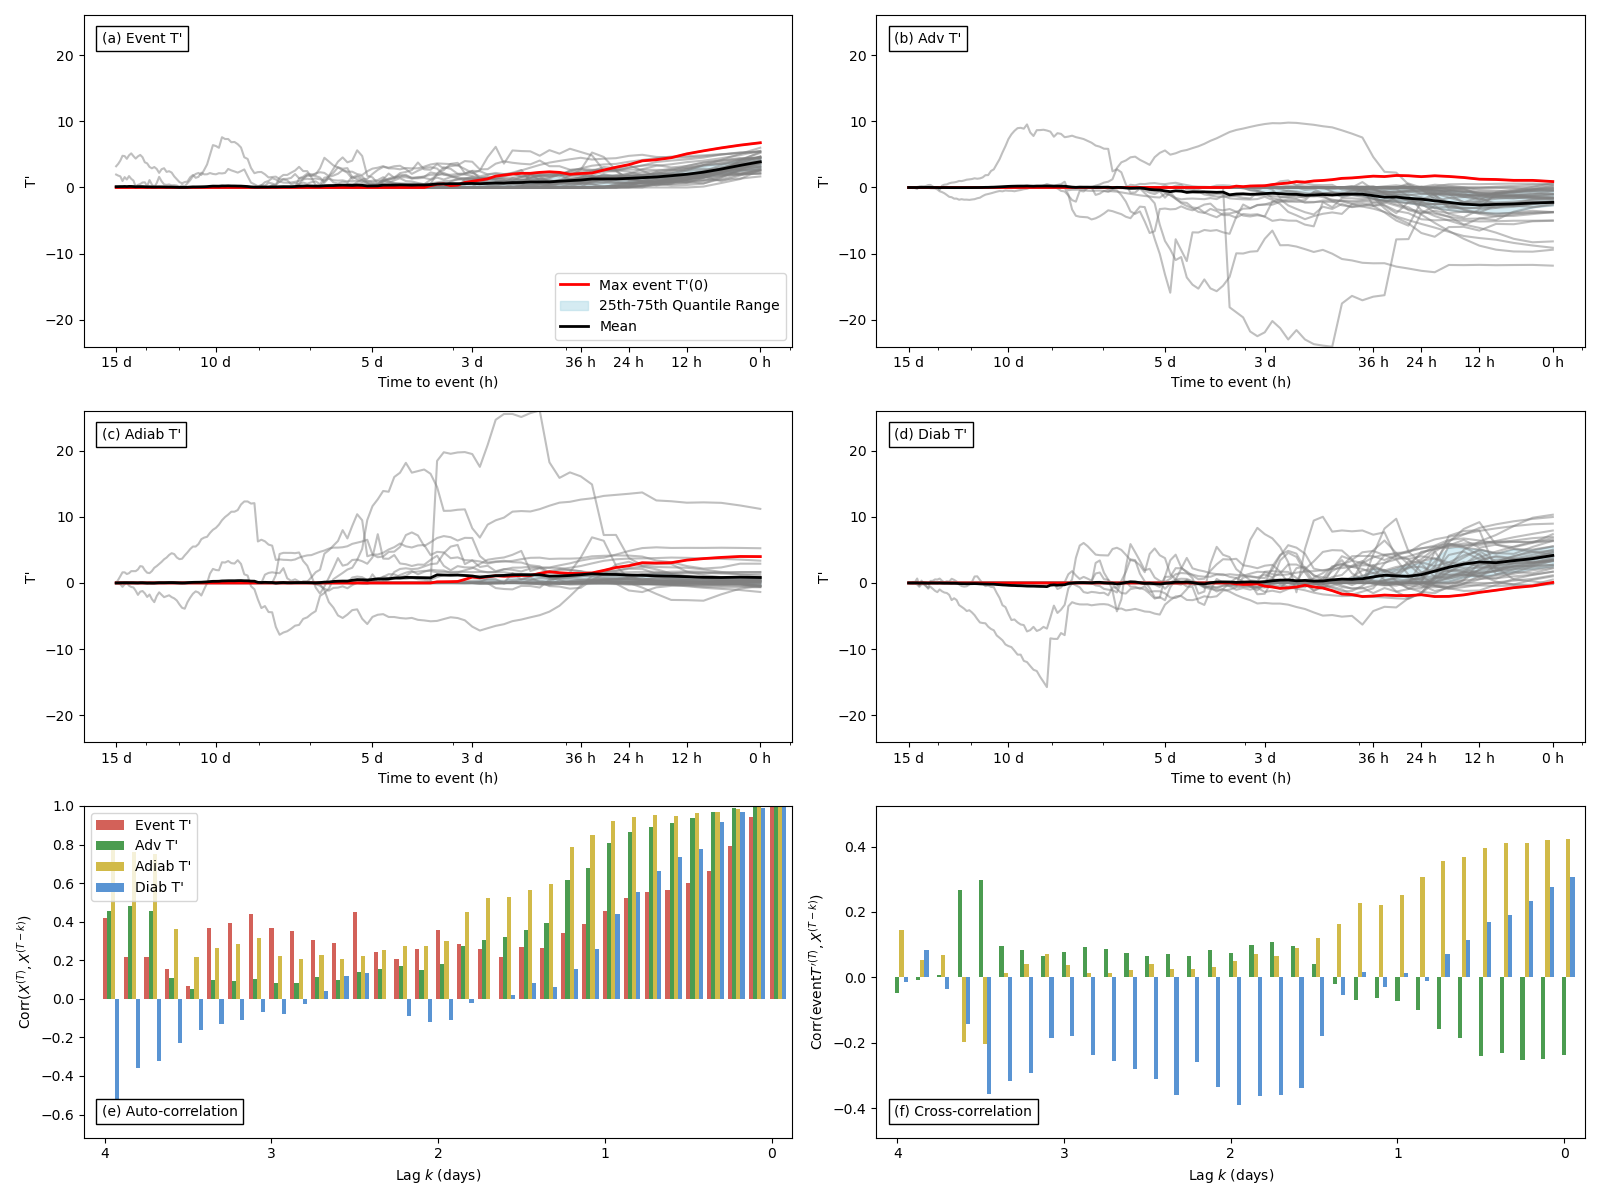
\includegraphics[width=0.9\textwidth]{images/sup1.png}
\end{figure}

\begin{figure}[h]
\caption{Location 45N 30W, in the middle of the Atlantic ocean.}
\centering
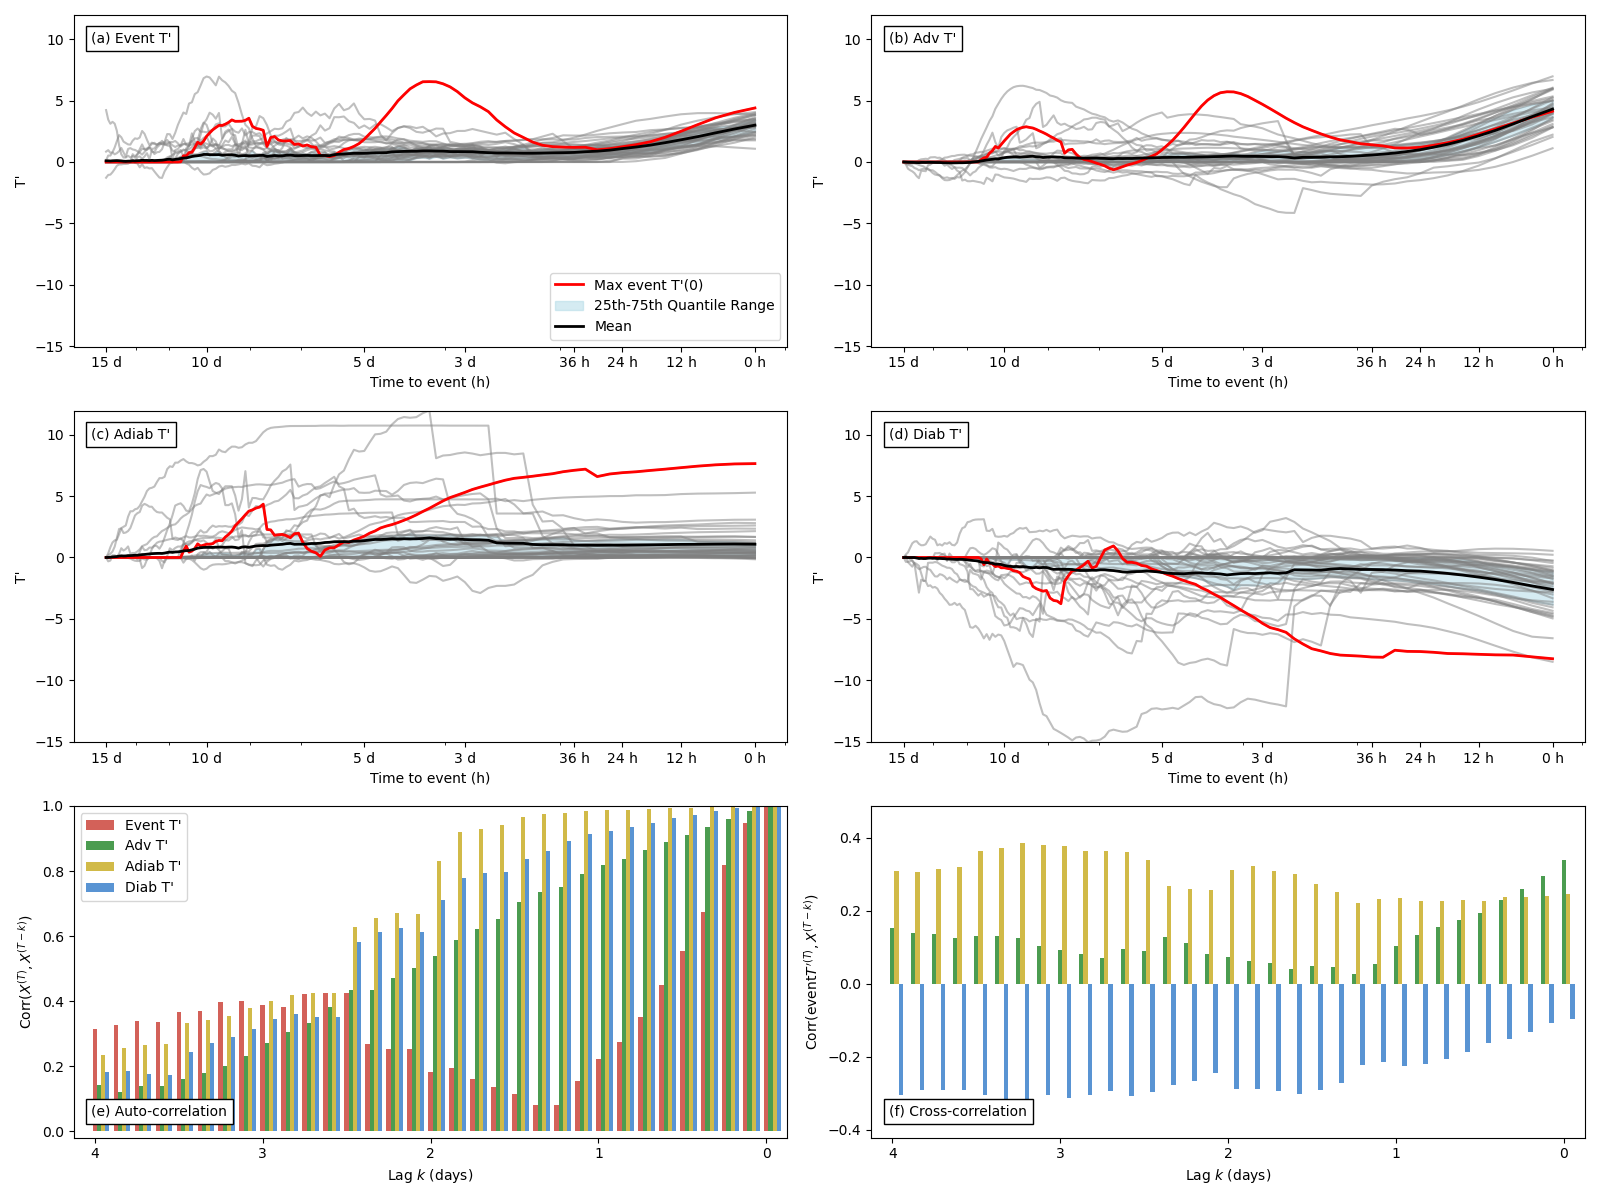
\includegraphics[width=0.9\textwidth]{images/sup2.png}
\end{figure}

\begin{figure}[h]
\caption{Location 32S 116E, in the vicinity of Perth, Australia.}
\centering
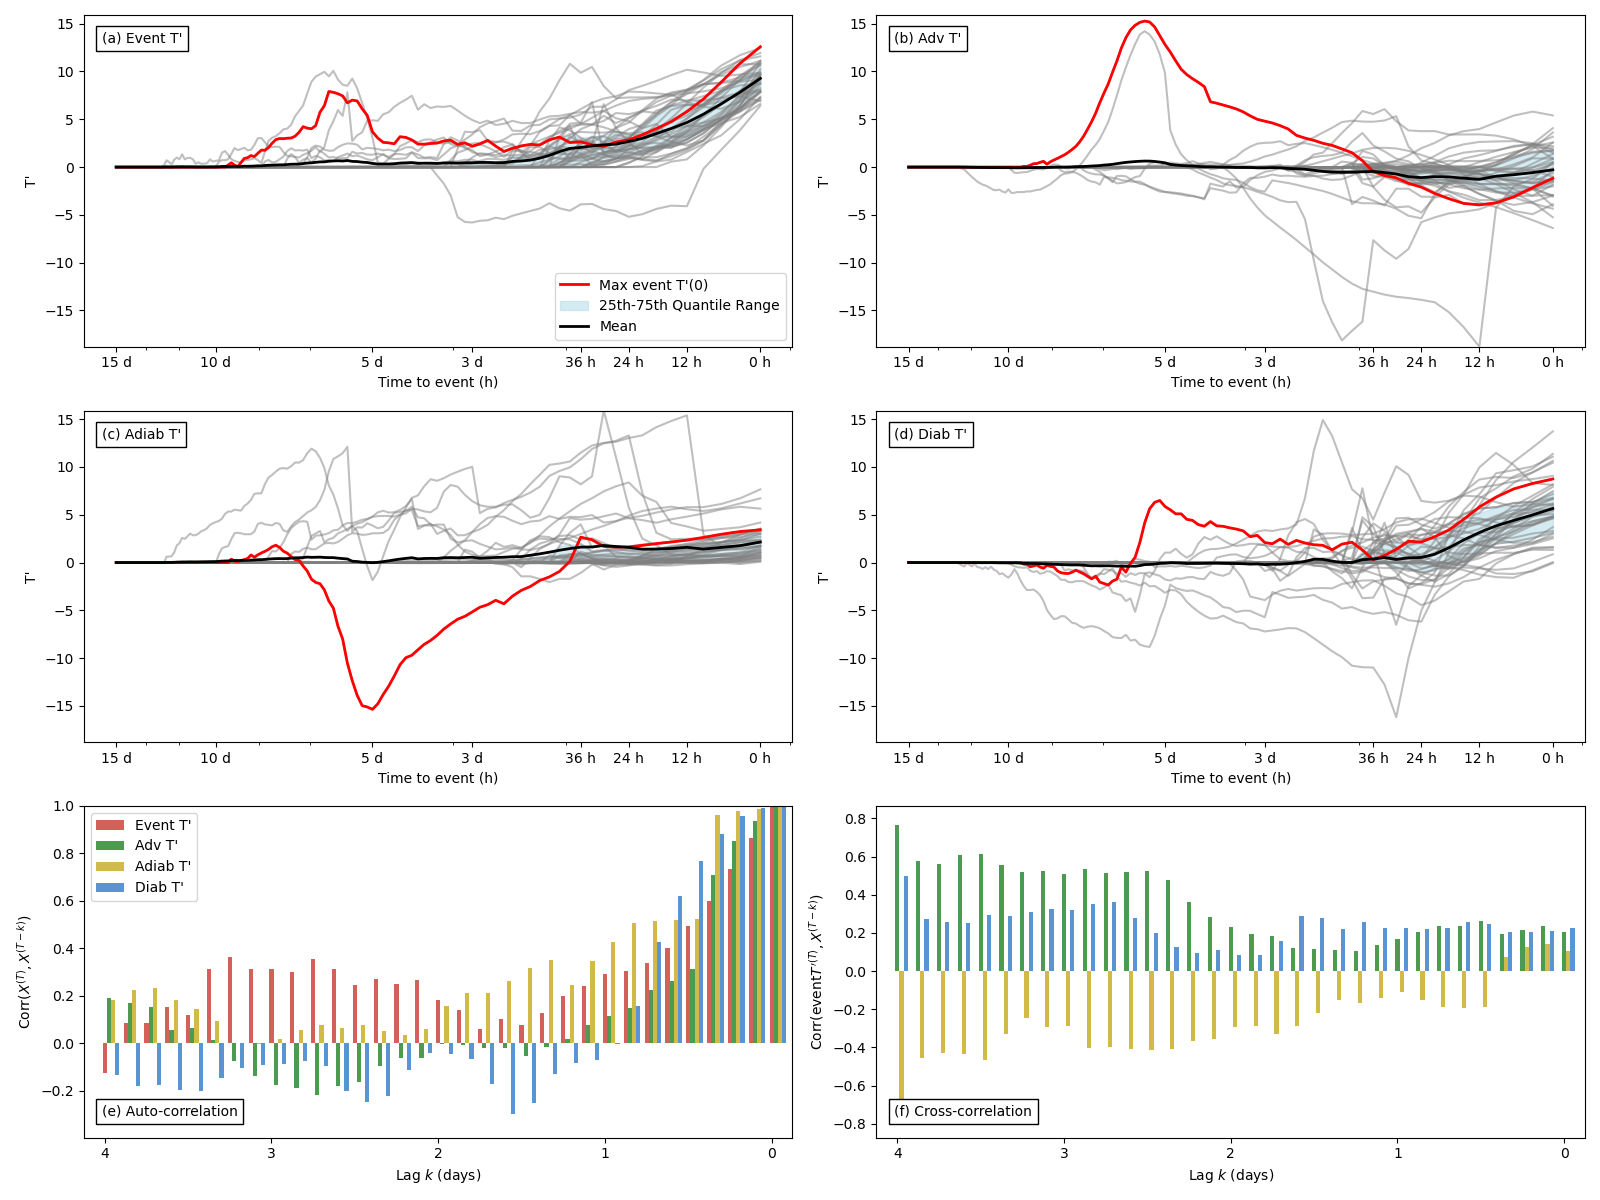
\includegraphics[width=0.9\textwidth]{images/sup3.png}
\end{figure}

\section{Differenced timeseries data}

%%% Local Variables: 
%%% mode: latex
%%% TeX-master: "MasterThesisSfS"
%%% End: 

\chapter{Yet another appendix....}

\section{Description}
\begin{description}
\item[Something] details.
\item[Something else] other definition.
\end{description}

\section{Tables}
Refer to Table~\ref{tab:example} to see a left justified table with caption
on top.

\begin{table}[ht]
\centering
\caption[Test results]{\label{tab:example}Results.}
\begin{tabular}{ll}
\hline
\textbf{Student} & \textbf{Grade}\\
\hline
Marie  & $6$\\
Alain  & $5.5$\\
Josette  & $4.5$\\
Pierre  & $5$\\
\hline
\end{tabular}
\end{table}

%%% Local Variables: 
%%% mode: latex
%%% TeX-master: "MasterThesisSfS"
%%% End: 



%% Epilogue (optional)
\addtocontents{toc}{\vspace{.5\baselineskip}}
\cleardoublepage
\phantomsection

\markboth{Epilogue}{Epilogue}
\chapter*{Epilogue}
\label{s:Epilogue}

A few final words.



%%% Local Variables: 
%%% mode: latex
%%% TeX-master: "MasterThesisSfS"
%%% End: 



%%%%%%%%%%%%%%%%%%%%%%%%%%%%%%%%%%%%%%%%%%%%%%%%%%
%%% Declaration of originality (Do not remove!)%%%
%%%%%%%%%%%%%%%%%%%%%%%%%%%%%%%%%%%%%%%%%%%%%%%%%%
%% Instructions:
%% -------------
%% fill in the empty document confirmation-originality.pdf electronically
%% print it out and sign it
%% scan it in again and save the scan in this directory with name
%% confirmation-originality-scan.pdf
%%
%% General info on plagiarism:
%% https://www.ethz.ch/students/en/studies/performance-assessments/plagiarism.html
\cleardoublepage
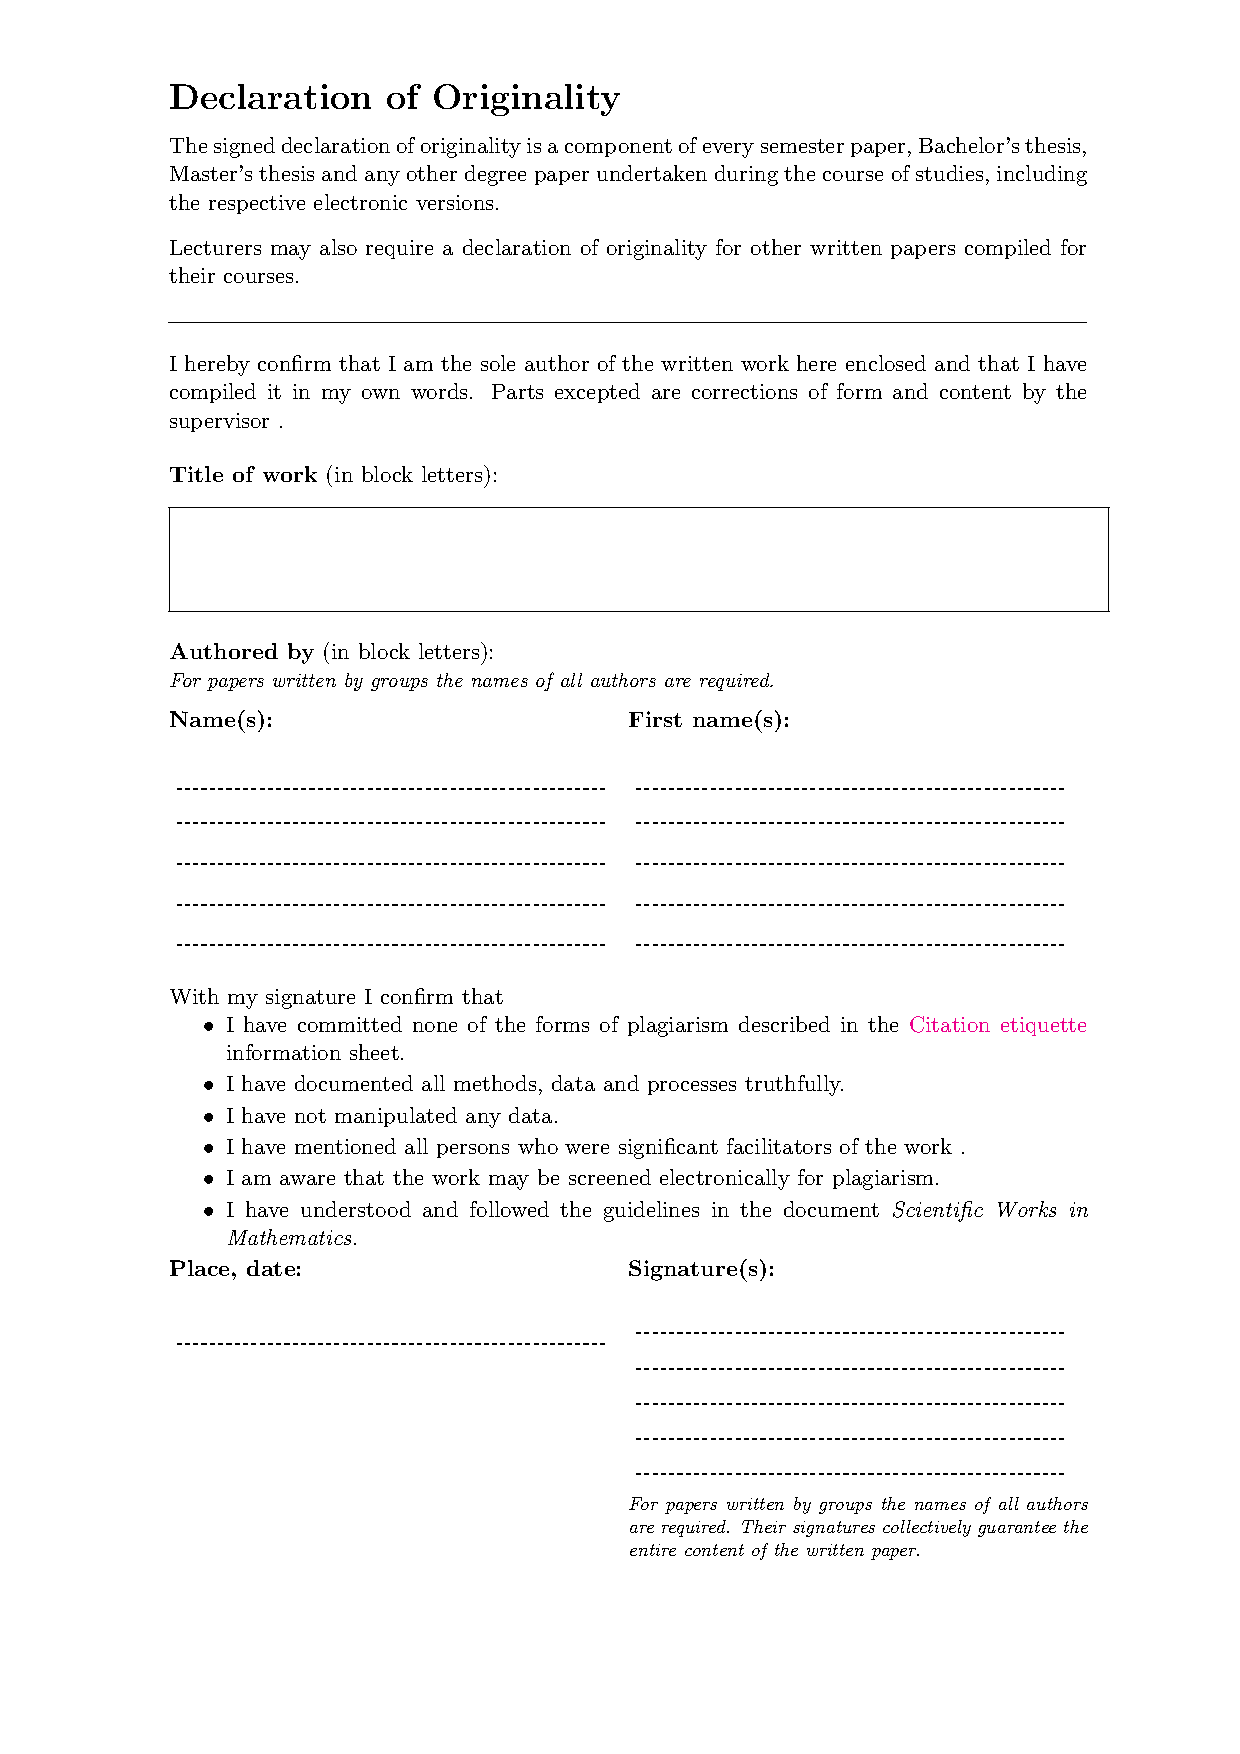
\includepdf[pages={-}, frame=true,scale=1]{pdf/confirmation-originality.pdf}
\end{document}
